% % % % % % % % % % % % % % % % % % % % % % % % % % % % % % % % % % % % % % % % % % % %
%                                                                                     %
% Short Sectioned Assignment LaTeX Template Version 1.0 (5/5/12)                      %
% This template has been downloaded from: http://www.LaTeXTemplates.com               %
%                                                                                     %
% Original author:  Frits Wenneker (http://www.howtotex.com)                          %
%                                                                                     %
% Modified by: Fco Javier Sueza Rodríguez (fcosueza@disroot.org)                      %
%                                                                                     %
% Changes:                                                                            %
%	    - Custom Chapters, Sections and Subsections (titlesec package)                %
%           - Document type scrbook (oneside)                                         %
%           - Use babel-lang-spanish package and marvosym                             %
%           - Use hyperref, enumitem, tcolorbox and glossaries packages               %
%           - Use Time New Roman (mathptmx), Helvetic and Courier fonts               %
%                                                                                     %
% License: CC BY-NC-SA 3.0 (http://creativecommons.org/licenses/by-nc-sa/3.0/)        %
%                                                                                     %
% % % % % % % % % % % % % % % % % % % % % % % % % % % % % % % % % % % % % % % % % % % %

%-----------------------------------------------%
%	              Packages                  %
%-----------------------------------------------%

\documentclass[paper=a4, fontsize=11pt, oneside]{scrbook}

% ---- Text Input/Output ----- %

\usepackage[T1]{fontenc}
\usepackage[utf8]{inputenc}
\usepackage{mathptmx}
\usepackage[scaled=.92]{helvet}
\usepackage{courier}
\usepackage[indent=12pt]{parskip}

\usepackage{geometry}
\geometry{verbose,tmargin=3cm,bmargin=3cm,lmargin=2.6cm,rmargin=2.6cm}

% ---- Language ----- %

\usepackage[spanish]{babel}
\usepackage{marvosym}

% ---- Another packages ---- %

\usepackage{amsmath,amsfonts,amsthm}
\usepackage{graphics,graphicx}
\usepackage{titlesec}
\usepackage{fancyhdr}
\usepackage{tcolorbox}
\usepackage{hyperref}
\usepackage{enumitem}
\usepackage[automake]{glossaries}

%--------------------------------------------------------------------%
%                      Customizing Document                          %
%--------------------------------------------------------------------%


% ----------- Custom Chapters, Sections and Subsections -------------- %

\titleformat{\chapter}[display]
			{\bfseries\Huge}
			{Tema \ \thechapter} {0.5ex}
			{\vspace{1ex}\centering}

\titleformat{\section}[hang]
			{\bfseries\Large}
			{\thesection}{0.5em}{}

\titleformat{\subsection}[hang]
			{\bfseries\large}
			{\thesubsection}{0.5em}{}

\titleformat{\subsubsection}[hang]
			{\bfseries\large}
			{\thesubsubsection}{0.5em}{}

\hypersetup{
    colorlinks=true,
    linkcolor=black,
    urlcolor=magenta
}

% ------------------- Custom heaaders and footers ------------------- %

\pagestyle{fancyplain}

\fancyhead[]{}
\fancyfoot[L]{}
\fancyfoot[C]{}
\fancyfoot[R]{\thepage}

\renewcommand{\headrulewidth}{0pt} % Remove header underlines
\renewcommand{\footrulewidth}{0pt} % Remove footer underlines

\setlength{\headheight}{13.6pt} % Customize the height of the header

% --------- Numbering equations, figures and tables ----------------- %

\numberwithin{equation}{section} % Number equations within sections
\numberwithin{figure}{section} % Number figures within sections
\numberwithin{table}{section} % Number tables within sections

% ------------------------ New Commands ----------------------------- %

\newcommand{\horrule}[1]{\rule{\linewidth}{#1}} % Create horizontal rule command


%----------------------------------------------------------------------------------------
%	TÍTULO Y DATOS DEL ALUMNO
%----------------------------------------------------------------------------------------

\title{
\vspace{10ex}
\normalfont \normalsize
\huge \textbf{Tarea 4: Introducción al Posicionamiento SEO}
}
\author{Francisco Javier Sueza Rodríguez}
\date{\normalsize\today}

%----------------------------------------------------------------------------------------
%                                     DOCUMENTO
%----------------------------------------------------------------------------------------
\begin{document}

\maketitle

\thispagestyle{empty}

\vspace{65ex}

\begin{center}
    \begin{tabular}{l l}
        \textbf{Centro}: & IES Aguadulce \\
        \textbf{Ciclo Formativo}: & Desarrollo Aplicaciones Web (Distancia)\\
        \textbf{Asignatura}: & Horas de Libre Configuración\\
        \textbf{Tema}: & Tema 4 - Introducción al Posicionamiento SEO\\
    \end{tabular}
\end{center}

\newpage

\tableofcontents

\vspace{15ex}
\hrule
\vspace{10ex}


\listoffigures

\newpage

\section{Ejercicio 1}
Ahora vamos a  realizar una búsqueda en Google en este caso vamos a buscar \textbf{Desarrollo Web}. Una vez obtengas los resultados deberás realizar una captura de los resultados obtenidos y diferenciar sobre la misma los diferentes tipos de resultados que se obtienen: resultados de pago SEM, resultados SEO y resultados de shopping. algo parecido a lo que aparece en el punto 1 de la unidad. Una vez realizada explica brevemente la diferencia entre cada uno de ellos.

\subsection{Solución}
En este ejercicio se ha realizado una búsqueda en Google del término \textbf{comprar desarrollo web}, para que nos muestre todo tipo de resultados. Se ha tomado 2 capturas de pantallas para explicar un poco los resultados que hemos obtenido y de que tipo son cada uno.

\begin{figure}[H]
    \centering
    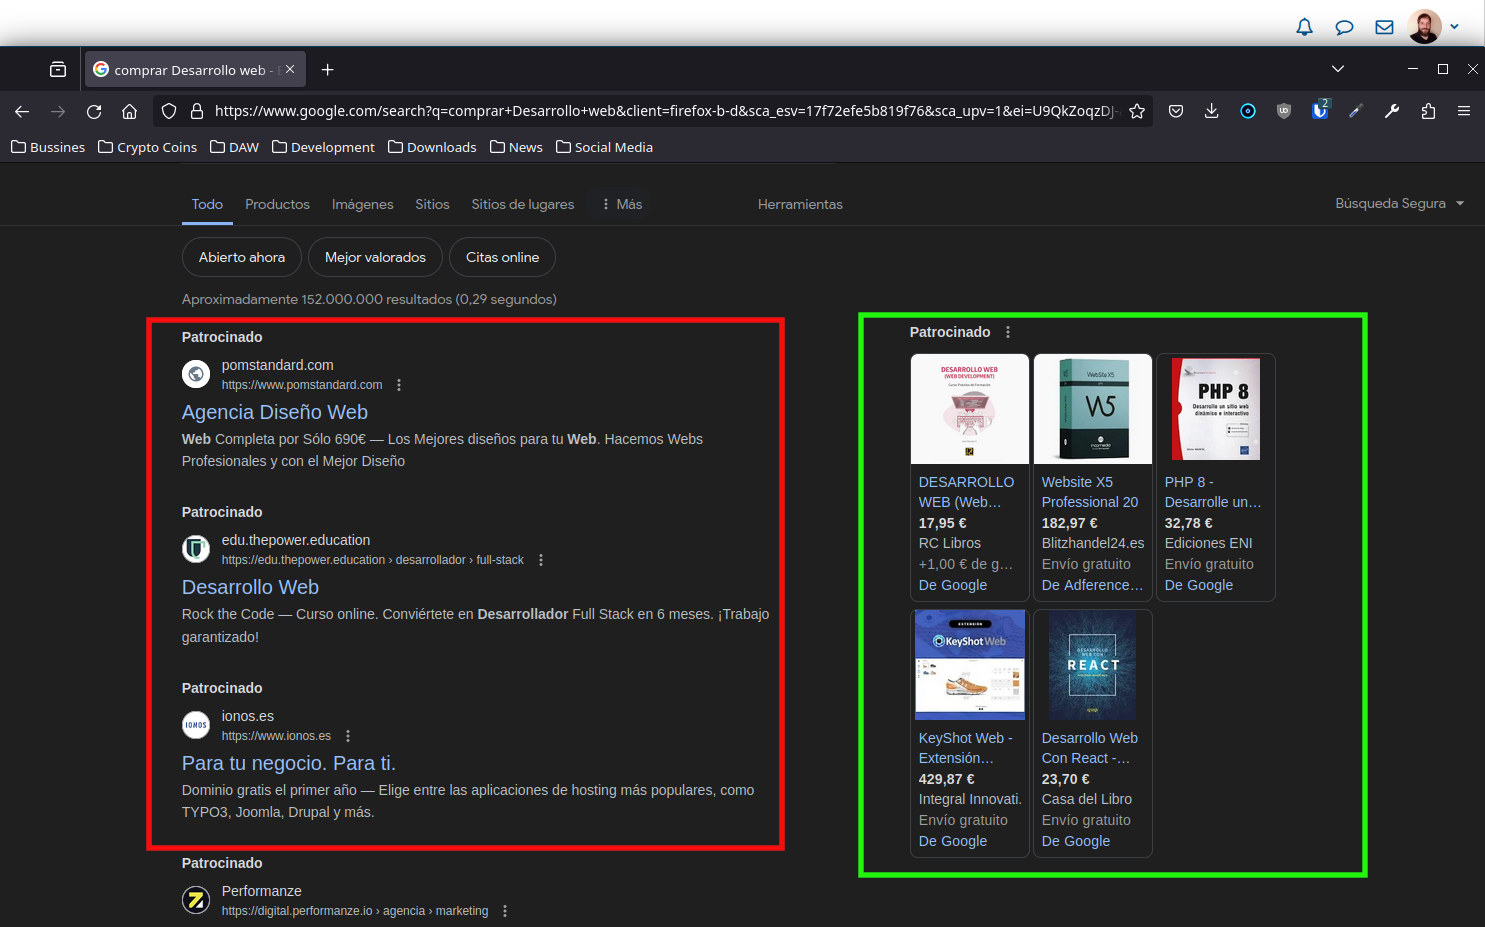
\includegraphics[scale=0.40]{search-1.png}
    \caption{Resultados patrocinados y shopping}
\end{figure}

En esta primera captura de la búsqueda podemos ver 2 tipos de resultados. Dentro de \textbf{recuadro rojo} podemos ver los resultado de \textbf{pago SEM}. Estos resultados que aparecen como promocionados por Google son resultado del pago, por parte de la webs, de un servicio de \textbf{SEM} (Search Engine Marketing), por el cual por un pago o cuota Google sitúa sus páginas web en los primeros resultados de búsqueda.

Por otro lado, dentro del \textbf{cuadrado verde}, tenemos los \textbf{resultados de Shopping}. En este caso, lo que se promociona no son webs, sino productos concretos, aunque la forma de proceder es parecida al SEM, ya que se paga una cuota a google (o pago único) para que con determinadas búsquedas sitúe nuestros productos en los resultados.

La\textbf{ diferencia} entre los resultados \textbf{SEM y Shopping} es que mientras que los primeros están \textbf{orientado a promocionar sitios web}, el segundo esta \textbf{orientado a productos concretos}.

\begin{figure}[H]
    \centering
    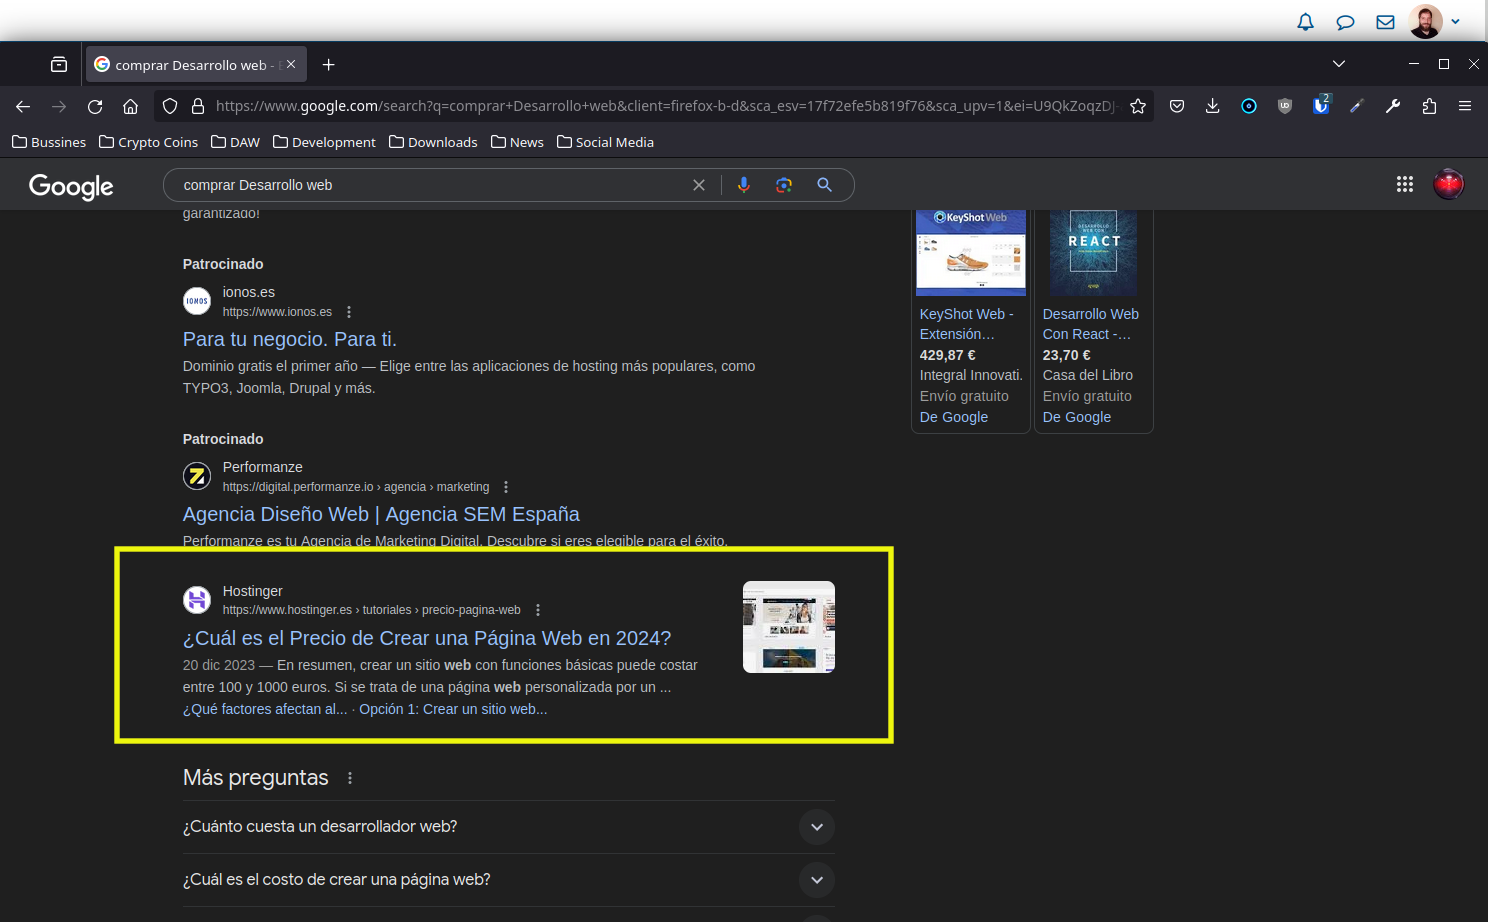
\includegraphics[scale=0.40]{search-2.png}
    \caption{Resultados SEO}
\end{figure}

En esta segunda captura, se muestra la segunda parte de la búsqueda donde aparecen los \textbf{resultados SEO}, dentro del \textbf{rectángulo amarillo}. Estos resultados se ordenan estrictamente por las diferentes técnicas de posicionamiento SEO que se hayan usado en el desarrollo de la web, como la inclusión de palabras claves en textos de la propia web, palabras en el tag \textbf{meta description} o \textbf{meta keyword}, etc...

\section{Ejercicio 2}
Utiliza la herramienta \href{https://trends.google.es/trends/}{Google Trends} y encuentra las siguientes tendencias:
\begin{itemize}
    \item Tendencia en España en el último día en la categoría Informática y telecomunicaciones, búsqueda web.
    \item Tendencia en España en los últimos 7 días  en la categoría viajes, búsqueda web.
\end{itemize}

\subsection{Solución}
En este ejercicio vamos a usar \textbf{Google Trends} para consultar la tendencias de búsqueda en España sobre diferentes temas y durante diferentes períodos de tiempo.

En primer lugar, hemos consultado la \textbf{tendencia del último día} relacionada con \textbf{informática y electrónica} y también con \textbf{internet y telecomunicaciones}.

Como podemos ver en las 2 gráficas las tendencias son parecidas en ambos temas, con caídas durante las horas de madrugada y búsquedas mucho más activas el resto del día, llegando ambos temas a \textbf{popularidad máxima} sobre las \textbf{12h} de la mañana. A continuación vemos 2 capturas con los resultados de la búsqueda en Google Trends.

\begin{figure}[H]
    \centering
    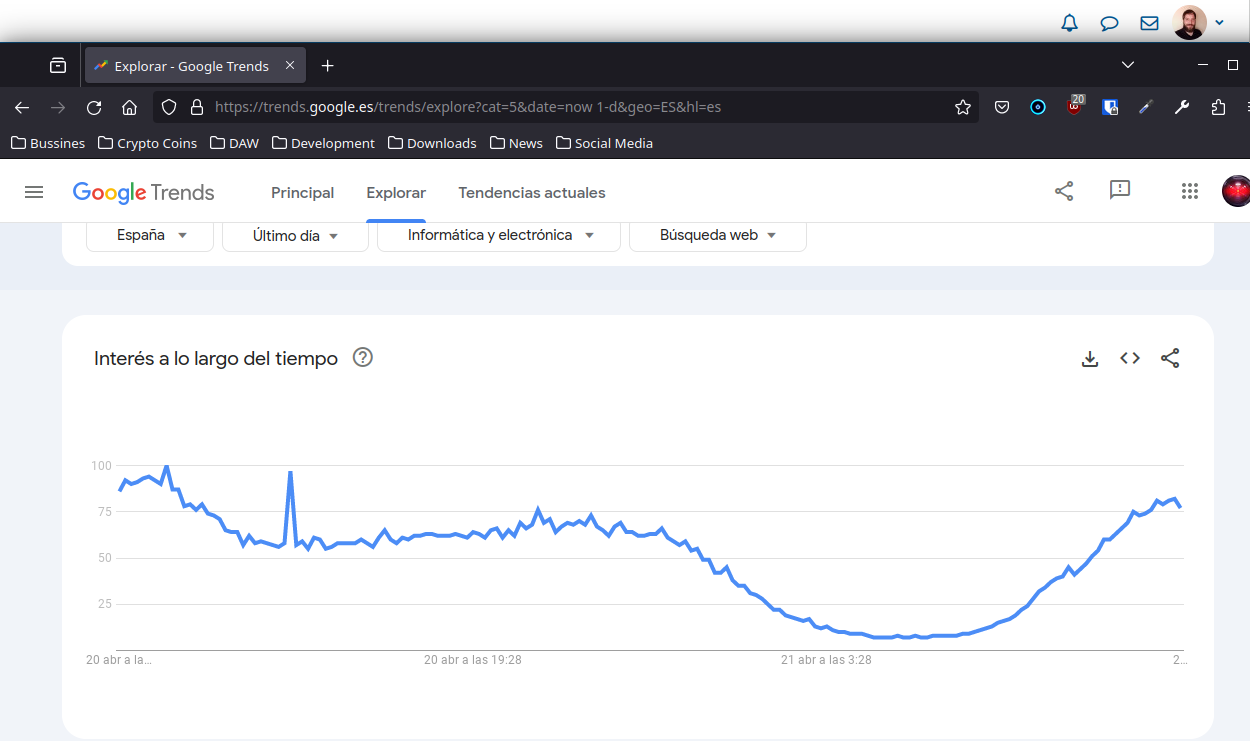
\includegraphics[scale=0.40]{trends-1.png}
    \caption{Tendencia de Informática y Electrónica en el último día}
\end{figure}

\begin{figure}[H]
    \centering
    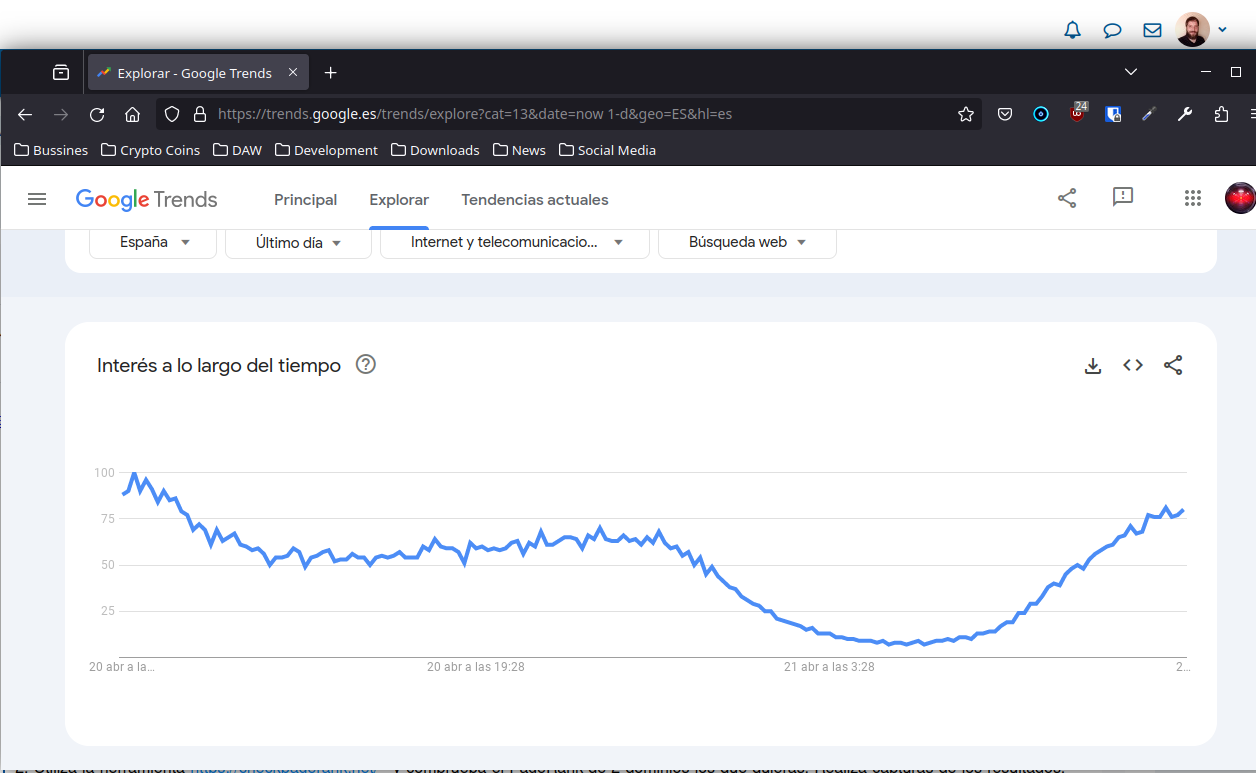
\includegraphics[scale=0.40]{trends-2.png}
    \caption{Tendencia de Internet y Telecomunicaciones en el último día}
\end{figure}

En segundo lugar hemos obtenido la \textbf{tendencia de los últimos 7 días} de las búsquedas realizadas sobre \textbf{viajes}.

Como podemos ver, la popularidad de este tema es menor que la de los temas anteriores, ya que en la última semana solo ha habido un día en el que se ha llegado a una popularidad del 100, mientras que los temas anteriores han llegado casi a diario y alguno hasta varias veces en un mismo día.

En la siguiente captura podemos ver la gráfica de esta tendencia.

\begin{figure}[H]
    \centering
    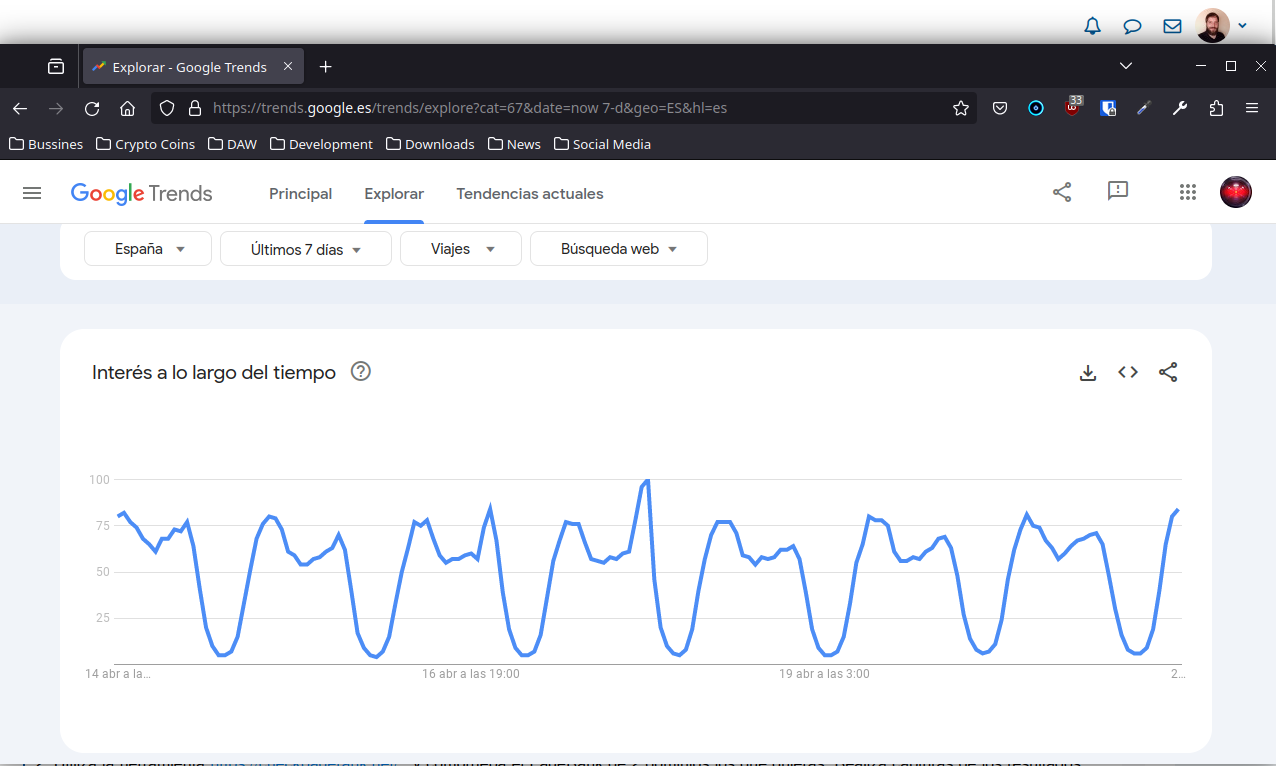
\includegraphics[scale=0.40]{trends-3.png}
    \caption{Tendencia de Viajes en los últimos 7 días}
\end{figure}

\section{Ejercicio 3}
Utiliza la herramienta \href{https://checkpagerank.net/}{Checkpagerank}  y comprueba el PageRank de 2 dominios los que quieras. Realiza capturas de los resultados. Intenta elegir páginas que sepas que son muy visitadas para que veas que el Pagerank se mide correctamente.

\subsection{Solución}
En primer lugar se ha consultado el PageRank de la web \url{store.steampowered.com}, uno de los sitios web de venta de
videojuegos más visitados a nivel mundial. Como vemos, las métricas que arroja la búsqueda son muy altas, indicando el
gran posicionamiento de esta web.

\begin{figure}[H]
    \centering
    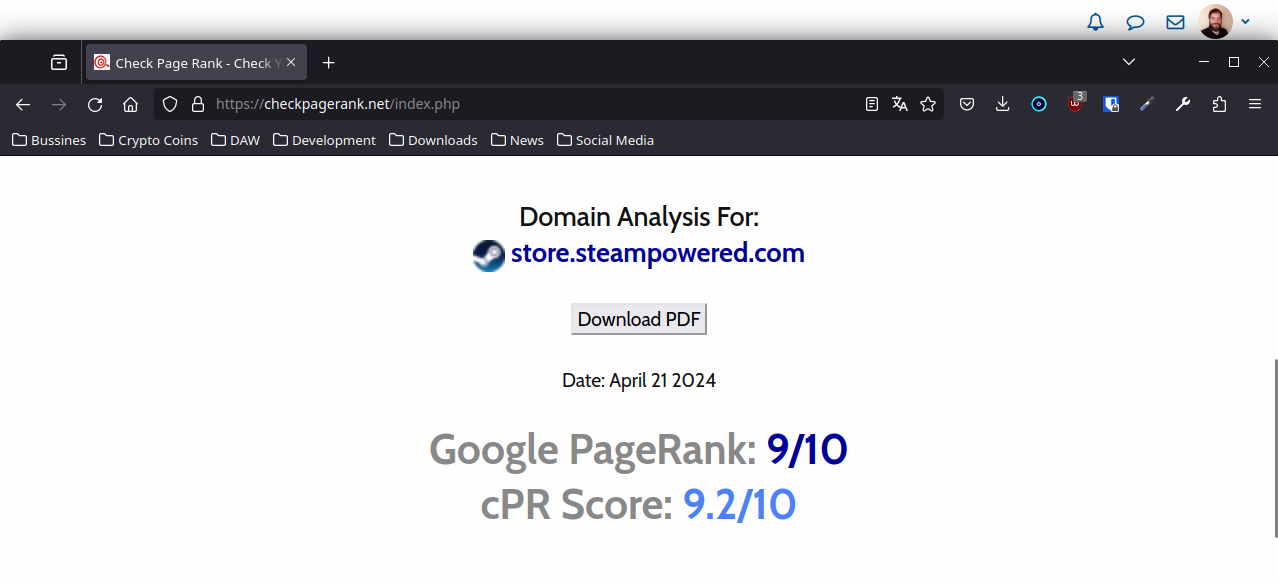
\includegraphics[scale=0.40]{rank-1.png}
    \caption{PageRank para la web store.steampowered}
\end{figure}

La segunda web consultada ha sido sobre la página \url{www.nytimes.com}, la página principal de The New York Times, uno de los periódicos más consultados a nivel mundial. Como vemos en la captura, las métricas de esta web son incluso superiores a las del store de Steam, algo que tampoco sorprende.

\begin{figure}[H]
    \centering
    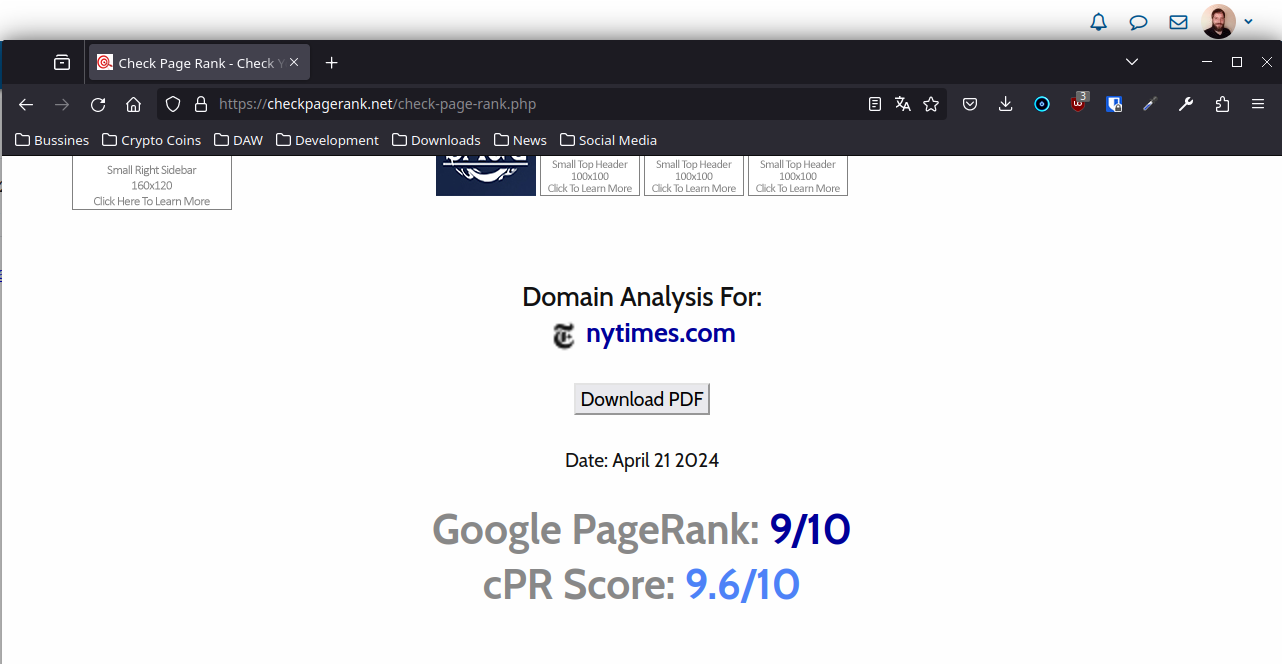
\includegraphics[scale=0.40]{rank-2.png}
    \caption{PageRank para la web del New York Times}
\end{figure}

\section{Ejercicio 4}
Utiliza el blog que creaste en la unidad 1 e inserta  un par de entradas más o si no lo tienes crea uno,  son unos simples pasos con Blogger. Si tienes un sitio web también puedes hacer el ejercicio con él.

\begin{itemize}
    \item Genera el sitemap del sitio web o de tu blog con la herramienta del punto 3.1.3 del debes conocer.
    \item ¿Cuál crees que sería un buen tittle para tu sitio? Utiliza el contador de caracteres SEO del punto 3.1.5 de la unidad.
\end{itemize}

\subsection{Solución}
En este último apartado vamos a trabajar sobre el sitio web que se desarrollo en la tarea 1 de la asignatura. En mi caso fue el sitio de una la empresa ficticia \href{https://sites.google.com/view/sitewise/inicio}{SiteWISE}.

En primer lugar, vamos a generar un sitemap con la herramienta \href{https://www.xml-sitemaps.com/}{XML-Sitemaps}, como se indica en el punto 3.1.3 de la teoría de este tema.

Después de introducir la dirección en la herramienta, se ha generado el sitemap, que podemos ver resumido en la siguiente captura, de forma correcta e indicando la prioridad de cada una de las secciones del sitio web. Adicionalmente, se nos muestra información interesante a la derecha, como la fecha de creación de la página web, si contiene enlaces rotos, etc. En el Anexo A se incluye el código XML generado.


\begin{figure}[H]
    \centering
    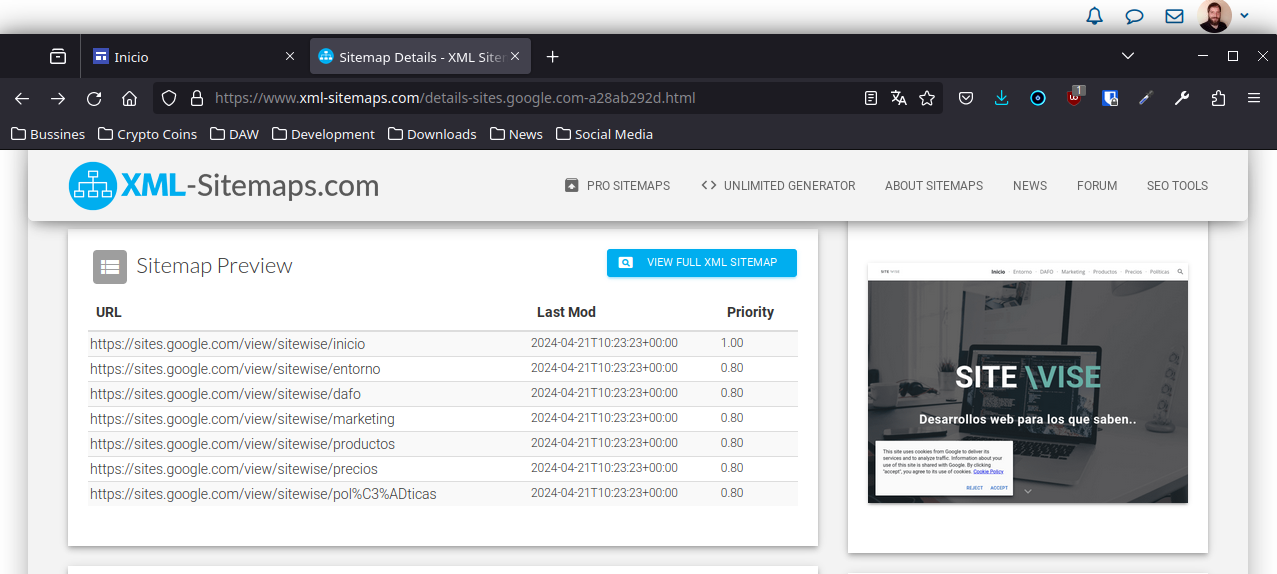
\includegraphics[scale=0.40]{sitemap.png}
    \caption{Sitemap del sitio web de SiteWISE}
\end{figure}

En según y último lugar vamos a usar el \href{https://www.contadordecaracteres.com/contador-de-caracteres-para-seo.html}{contador de carácteres SEO} que se indican en el apartado 3.1.5 de los apuntes de este tema. En la siguiente captura, podemos ver cual ha sido el resultado después de introducir los diferentes textos que nos podrían ayudar para el SEO de nuestra página.

\begin{figure}[H]
    \centering
    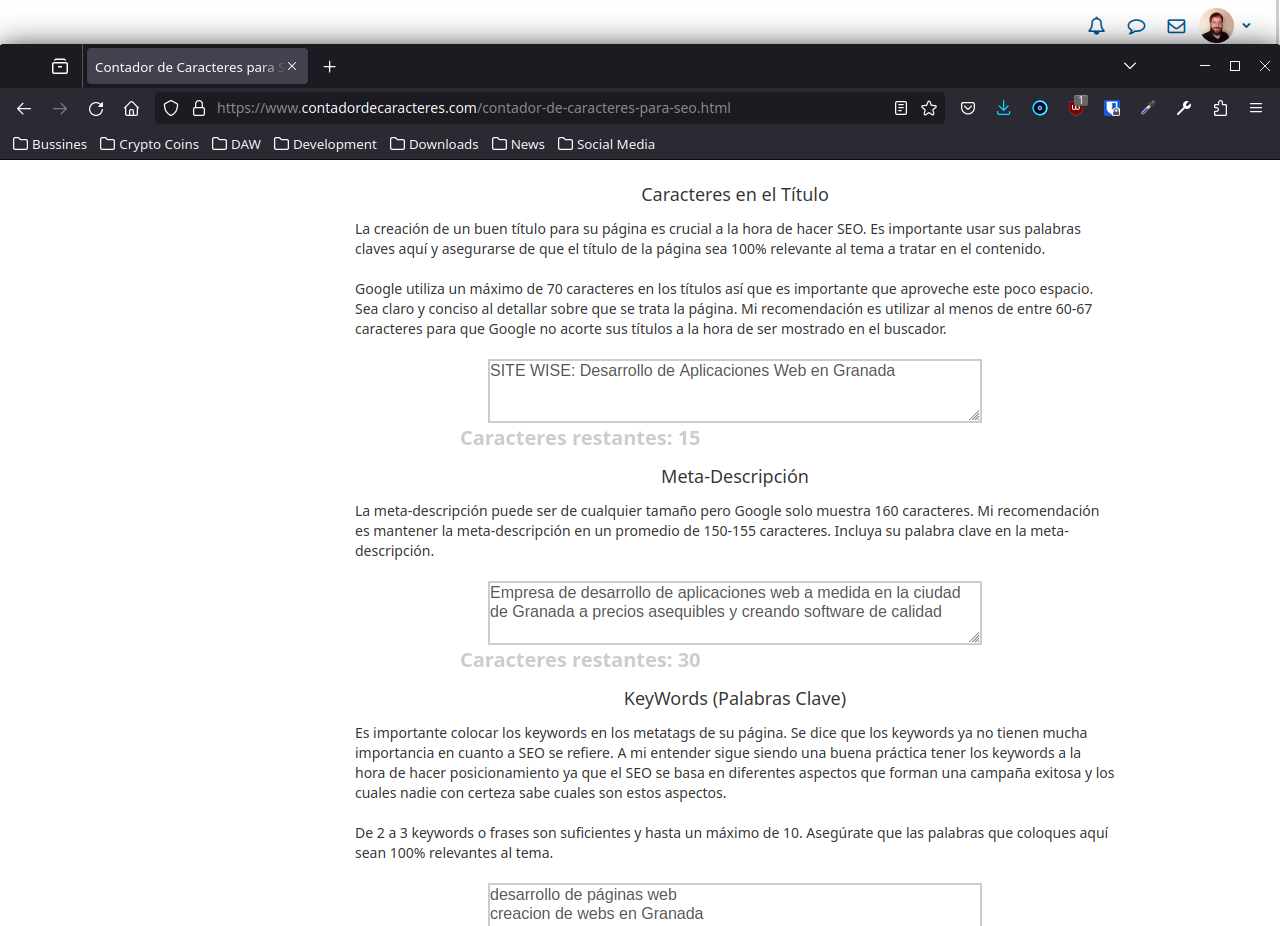
\includegraphics[scale=0.40]{seo.png}
    \caption{Uso del contador de caracteres SEO}
\end{figure}

Como se ve en la captura, un \textbf{buen título} para el sitio web sería el de \textbf{SITEWISE: Desarrollo de Aplicaciones Web en Granada}, ya que es un título que incluye el nombre de la empresa así como la descripción de su principal servicio y su ubicación, llegando además casi a los 60 caracteres recomendados.

\appendix

\section{Código XML con el sitemap generado}
\begin{figure}[H]
    \begin{tcolorbox}[sharp corners, colback=yellow!30, colframe=white!20]
        \scriptsize
        \begin{verbatim}
<urlset xmlns="http://www.sitemaps.org/schemas/sitemap/0.9"
        xmlns:xsi="http://www.w3.org/2001/XMLSchema-instance"
       xsi:schemaLocation="http://www.sitemaps.org/schemas/sitemap/0.9
                           http://www.sitemaps.org/schemas/sitemap/0.9/sitemap.xsd">

<!--  created with Free Online Sitemap Generator www.xml-sitemaps.com  -->

    <url>
        <loc>https://sites.google.com/view/sitewise/inicio</loc>
        <lastmod>2024-04-21T10:23:23+00:00</lastmod>
        <priority>1.00</priority>
    </url>
    <url>
        <loc>https://sites.google.com/view/sitewise/entorno</loc>
        <lastmod>2024-04-21T10:23:23+00:00</lastmod>
        <priority>0.80</priority>
    </url>
    <url>
        <loc>https://sites.google.com/view/sitewise/dafo</loc>
        <lastmod>2024-04-21T10:23:23+00:00</lastmod>
        <priority>0.80</priority>
    </url>
    <url>
        <loc>https://sites.google.com/view/sitewise/marketing</loc>
        <lastmod>2024-04-21T10:23:23+00:00</lastmod>
    <priority>0.80</priority>
    </url>
    <url>
        <loc>https://sites.google.com/view/sitewise/productos</loc>
        <lastmod>2024-04-21T10:23:23+00:00</lastmod>
        <priority>0.80</priority>
    </url>
    <url>
        <loc>https://sites.google.com/view/sitewise/precios</loc>
        <lastmod>2024-04-21T10:23:23+00:00</lastmod>
        <priority>0.80</priority>
    </url>
    <url>
        <loc>https://sites.google.com/view/sitewise/pol%C3%ADticas</loc>
        <lastmod>2024-04-21T10:23:23+00:00</lastmod>
        <priority>0.80</priority>
    </url>
</urlset>
        \end{verbatim}
    \end{tcolorbox}
\end{figure}

% Bibliography

%\newpage
%\bibliography{citas}
%\bibliographystyle{unsrt}

\end{document}